% Template for Cogsci submission with R Markdown

% Stuff changed from original Markdown PLOS Template
\documentclass[10pt, letterpaper]{article}

\usepackage{cogsci}
\usepackage{pslatex}
\usepackage{float}
\usepackage{caption}

% amsmath package, useful for mathematical formulas
\usepackage{amsmath}

% amssymb package, useful for mathematical symbols
\usepackage{amssymb}

% hyperref package, useful for hyperlinks
\usepackage{hyperref}

% graphicx package, useful for including eps and pdf graphics
% include graphics with the command \includegraphics
\usepackage{graphicx}

% Sweave(-like)
\usepackage{fancyvrb}
\DefineVerbatimEnvironment{Sinput}{Verbatim}{fontshape=sl}
\DefineVerbatimEnvironment{Soutput}{Verbatim}{}
\DefineVerbatimEnvironment{Scode}{Verbatim}{fontshape=sl}
\newenvironment{Schunk}{}{}
\DefineVerbatimEnvironment{Code}{Verbatim}{}
\DefineVerbatimEnvironment{CodeInput}{Verbatim}{fontshape=sl}
\DefineVerbatimEnvironment{CodeOutput}{Verbatim}{}
\newenvironment{CodeChunk}{}{}

% cite package, to clean up citations in the main text. Do not remove.
\usepackage{cite}

\usepackage{color}

% Use doublespacing - comment out for single spacing
%\usepackage{setspace}
%\doublespacing


% % Text layout
% \topmargin 0.0cm
% \oddsidemargin 0.5cm
% \evensidemargin 0.5cm
% \textwidth 16cm
% \textheight 21cm

\title{Word Learning as Network Growth: a Cross-linguistic Analysis}


\author{{\large \bf Abdellah Fourtassi} \\ \texttt{afourtas@stanford.edu} \\ Department of Psychology \\ Stanford University \And {\large \bf Yuan Bian} \\ \texttt{ybian.uiuc@gmail.com} \\ Department of Psychology \\ University of Illinois \And {\large \bf Michael C. Frank} \\ \texttt{mcfrank@stanford.edu} \\ Department of Psychology \\ Stanford University}

\begin{document}

\maketitle

\begin{abstract}
Children tend to learn first the words that are highly connected in the
lexical network (i.e., words that are connected to a variety of other
words). The process by which connectivity in both the phonological and
semantic netwoks come to influence word learning is still not very well
understood. One view suggests that learning is driven primarily by
\emph{internal} connectivity in the child's available lexicon. Another
view suggests that \emph{external} connectivity in the learning
environment is what makes words salient and readily learned. The present
study tests both scenarios systematically in both the phonological and
the the semantic domains, and across 8 languages. We generate the
results obtained by Hills et al. (2009) with English semantic networks,
and show that external connectivity in the learning environment, rather
than internal connectivity, drives growth of both semantic and
phonological networks. Finally, we demonstrate that these effects hold
cross-linguistically.

\textbf{Keywords:}
semantic network, phonological network, word learning
\end{abstract}

\section{Introduction}\label{introduction}

What factors shape vocabulary learning over the course of early
childhood? To investigate this question, scientists have adopted
multiple research strategies, from controlled laboratory experiments to
corpus analysis. One strategy consists in documenting the timeline of
words' acquisition, and studying the properies that make words easy or
hard to learn. For example, within a lexical category, words that are
more frequent in child-directed speech are acquired earlier (J. C.
Goodman, Dale, \& Li, 2008). Other factors include word length, the mean
length of utterances in which the word occurs, and how concrete the word
is (see Braginsky, Yurovsky, Marchman, \& Frank, 2016).

Besides these word-level properties, researchers found that the lexical
structure (that is, how words relate to each other) also influences the
age of acquisition of words. The lexical structure is best characterized
in terms of a network where each node represents a word in the
vocabulary, and each link between two nodes represents a relationship
between the corresponding pair of words. Previous studies investigated
early vocabulary networks based on different word relations such as
shared semantic features, target-cue relationship in free association
norms, co-occurrence in child directed speech, and phonological
similarity. These studies found that children tend to produce earlier
the words that have higher neighborhood density (i.g., high connectivity
in the network) both at the phonological and the semantic level
(Beckage, Smith, \& Hills, 2011; Engelthaler \& Hills, 2017; Hills,
Maouene, Riordan, \& Smith, 2010; Hills, Maouene, Maouene, Sheya, \&
Smith, 2009; Stella, Beckage, \& Brede, 2017; Stokes, 2010; Storkel,
2009).

A crucial question that naturally emerges from these analyses is how
does network connectivity influence word learning? Steyvers \& Tenenbaum
(2005) suggested that the effect of connectivity is the consequence of
how the lexical network gets constructed in the child's mind. According
to this explanation, known as Preferential Attachment (PAT), highly
connected words in the child's lexicon tend to ``attract'' more words
over time, in a rich-get-richer scenario (Barabasi \& Albert, 1999). In
other words, what predicts word learning is \emph{internal} connectivity
in the child's early lexicon. In contrast, Hills et al. (2009) found
that what biases the learning is not the connectivity in the child's
internal lexicon but, rather, \emph{external} connectivity in the
learning environment. They called this alternative explanation
Preferential Acquisition (PAC). Figure \ref{fig:growth} shows an
illustration of both growth scenarios with the same simplified network.

\begin{CodeChunk}
\begin{figure}[H]

{\centering 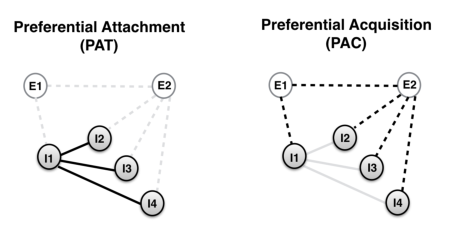
\includegraphics{figs/growth-1} 

}

\caption{\label{fig:growth}Illustration of the two growth models with the same network. Filled circles (I1-I4) represent known words (internal lexicon), and empty circles (E1 and E2) represent words that have not been learned yet (external lexicon). Black lines represent links that are relevant in each growth scenario, and gray lines represent links that are irrelevant. For PAT, each candidate node is characterized with the average degree (i.e., number of links) of the existing nodes that it would attach to. Thus, according to PAT, the node E1 is more likely to enter the lexicon first. For PAC, each candidate node is characterized with its degree in the entire network. According th PAC, the node E2 is more likely to enter the lexicon first.}\label{fig:growth}
\end{figure}
\end{CodeChunk}

Studies that investigted lexical network growth focused on semantic
networks using English data only (Hills et al., 2010, 2009; Steyvers \&
Tenenbaum, 2005). The novelty of the current study is that it
investigates whether phonological networks, like semantic networks, grow
by PAC, or if they rather grow by PAT. It also provides a systematic
comparision of network growth scenarios in both the phonological and the
semantic domains and assesses their relative contribution to the
learning process. Moreover, it tests the generality of the findings
across eight languages.

The paper is organized as follows. First, we describe the dataset we
used, the procedure we followed to construct both semantic and
phonological networks. Next, we show the results of the various analyses
we conducted comparing network growth scenarios across languages. Then
we test the overall contribution of the networks in the learning process
relative to other known predictors of age of acquisition (frequency and
length). Finally we discuss the major results in relation to known
experimental facts in language development.

\begin{CodeChunk}
\begin{figure*}[h]

{\centering 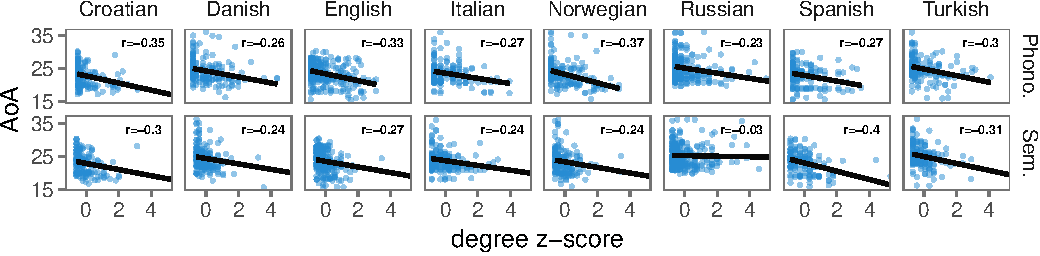
\includegraphics{figs/all_data-1} 

}

\caption{\label{fig:data_all}Age of acquisition in the end-state network as predicted by the degree in this network. Results are shown in each language for the phonological network (top) and the semantic network (bottom). Each point is a word, with lines indicating linear model fits.}\label{fig:all_data}
\end{figure*}
\end{CodeChunk}

\section{Networks}\label{networks}

\subsection{Data}\label{data}

We used data from Wordbank (Frank, Braginsky, Yurovsky, \& Marchman,
2017), an open repository aggregating cross-linguistic language
developmental data of the MacArthur-Bates Communicative Development
Inventory (CDI), a parent report vocabulary checklist. We used the
\emph{Words and Sentence} version of the CDI which contains the
productive vocabulary of toddlers (age varied between 16 to 36 months).
Following previous studies (Hills et al., 2009; e.g., Storkel, 2009), we
restricted our analysis to the category of nouns, since there are known
discrepancies between the learning of nouns, predicates, and function
words (e.g., Braginsky et al., 2016). The age of acquisition was defined
by the month at which a word was produced by at least 50\% of children
(J. C. Goodman et al., 2008).

We obtained these nouns in eight languages: Croatian, Danish, English,
Italian, Norwegian, Russian, Spanish, and Turkish. We used the subset of
nouns that had entries in the Florida Association Norms (see below).
Since these norms are available only in English, we used the translation
of non-English words provided by Braginsky et al. (2016). This allowed
us to use the English association norms across languages. Table
\ref{tab:stats} gives an overview of the data used. The translation of
non-English words is still an ongoing process. Note, however, that all
languages have at least 60\% of nouns translated.

\begin{table}[H]
\centering
\begin{tabular}{rlrrr}
  \hline
 & language & total & translated & normed \\ 
  \hline
1 & Croatian & 253 & 177 & 170 \\ 
  2 & Danish & 295 & 198 & 187 \\ 
  3 & English & 296 & 296 & 274 \\ 
  4 & Italian & 311 & 203 & 194 \\ 
  5 & Norwegian & 305 & 193 & 186 \\ 
  6 & Russian & 311 & 311 & 285 \\ 
  7 & Spanish & 240 & 173 & 163 \\ 
  8 & Turkish & 293 & 175 & 164 \\ 
   \hline
\end{tabular}
\caption{\label{tab:stats}Total number of productive nouns in the CDI (left). We used a subset of these nouns that had available English translations (middle). The final set consisted of nouns that had both available translations as well entries in the Free Association Norms (right).} 
\end{table}

With this data, we constructed both semantic and phonological networks.

\subsection{Semantic networks}\label{semantic-networks}

We used as an index of semantic relatedness the Florida Free Association
Norms (Nelson, McEvoy, \& Schreiber, 1998). This dataset was collected
by giving adult participants a word (the cue), and asking them to write
the first word that comes to mind (the target). For example, when given
the word ``ball'', they might answer with the word ``game''. A pair of
nodes were connected by a directed link from the cue to the target if
there was a cue-target relationship between these nodes in the
association norms. Each node was characterized by its ``indegree'',
which represents the number of links for which the word was the target.
Following Hills et al. (2009), we used as a proxy for the learning
environment, the network constructed using the full set of nouns in the
CDI data in each language (e.g., in English this corresponds to the
network by 30 months).

\subsection{Phonological networks}\label{phonological-networks}

We used as a measure of phonological relatedness between two nodes the
Levenshtein (edit) distance between their phonological forms. The
measure counts the minimum number of operations (insertions, deletions,
substitutions) required to change one string into another. We generated
approximate International Phonetic Alphabet (IPA) trnascriptions from
the orthographic transcription, across languages, using the open source
text-to-speech software
\textbf{\href{http://http://espeak.sourceforge.net/}{Espeak}.}

In previous studies, two nodes were linked if they had an edit distance
of 1 (Stokes, 2010; Storkel, 2009). However, in these previous studies
the network was built using an adult vocabulary. Here, similar to the
approximation we made for the semantic network, we used the full set of
nouns in the CDI data as a proxy for phonological connectivity in the
learning environment. However, since the children's vocabulary contains
very few word pairs with an edit distance of 1, the resulting network
was too sparse and uninformative. Thus, we increased the threshold from
1 to 2, that is, two node were related if their edit distance was equal
to 1 or 2. Each node was characterized with its degree, i.e., the number
of links it shares with other words.

\section{Analysis}\label{analysis}

We start by examining how connectivity in the global netowrk influences
the age of acqusition. Regardless of the growth mechanism that might
have given rise to this netowrk (i.e., PAC or PAT), we expect nodes with
the higher degrees in this network to be learned earlier than nodes with
the lower degrees. The network was constructed using nouns at the oldest
age for which we have CDI data. Figure \ref{fig:data_all} shows how the
age of acquisition for each word varies as a function of its degree (or
indegree for the semantic network). For ease of visual comparison, the
predictor (i.e., the degree) was centered and scaled across languages.
The plots show, overall, a negative correlation between the month of
acquisition and the degree, indicating that nouns with higher degrees
are generally learned earlier.

\begin{CodeChunk}
\begin{figure*}[h]

{\centering 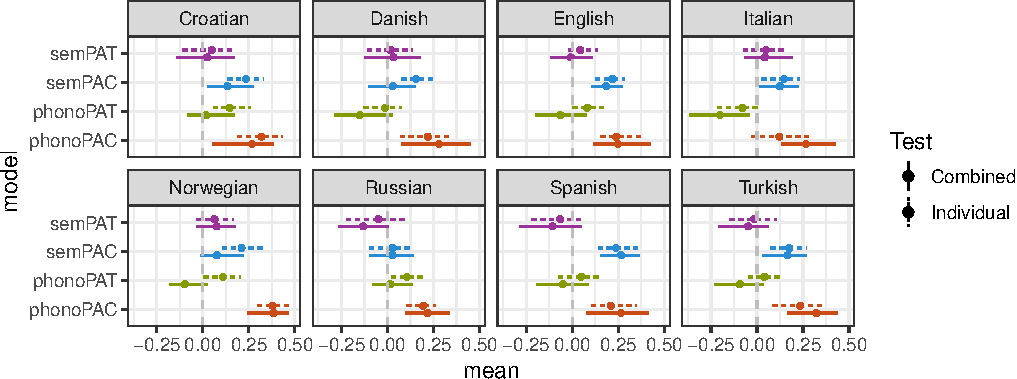
\includegraphics{figs/pred_ind_img-1} 

}

\caption{\label{fig:pred_ind}Evaluation of network growth scenarios both individually (dotted), and when combined in the same growth model (solid). Each dot represents the mean of the posterior distribution of the corresponding growth parameter, with ranges representing 95\% credible intervals (computed using the highest density intervals).}\label{fig:pred_ind_img}
\end{figure*}
\end{CodeChunk}

\subsection{Network growth models}\label{network-growth-models}

\subsubsection{How does each growth scenario predict noun
development?}\label{how-does-each-growth-scenario-predict-noun-development}

To test the network growth scenarios, we fit different growth models to
the data. We proceeded as follows. We calculated the probability that a
word \(w_i\), with a growth value \(d_i\) would enter the lexicon at a
given month, using a softmax function:

\begin{equation}
 p(w_i)= \frac{e^{\beta d_i}}{\sum_j e^{\beta d_j} }
\end{equation}

Where \(\beta\) is the fitting parameter. A positive value of \(\beta\)
means that words with higher growth values \(d_i\) are acquired first,
and a negative value means that words with lower growth values are
acquired first. As explained in Figure \ref{fig:growth}, each candidate
word \(w_i\) is characterized with a growth values \(d_i\) that depends
on the growth scenario tested. The normalization includes all words that
could be learned at that month.

We estimated the parameter \(\beta\) using a Bayesian approach. The
inference was performed using the probabilisitic programming language
WebPPL (N. Goodman \& Stuhlmüller, 2014). We started with a uniform
distribution, and at each month, we computed the likelihood function
over words that could possibly enter the lexicon at that month, fit to
the words that have been actually learned at that month (using formula
1). We ended up with a posterior distribution of \(\beta\), which we
summarized in Figure \ref{fig:pred_ind}.

Besides fitting a growth model to the data, we conducted another
evaluation. This second evaluation consists in determining, in each
month, the model-dependent growth value distribution of all words that
could possibly be learned at this month, and then computing the z-score
of each learned word with respect to this distribution. For each model,
we tested if the distribution constituted by the z-scores of all learned
words was different from zero, using a one-sample t-test.

The results from both evaluations were very similar and lead essentially
to the same
conclusions\footnote{we do not show here the resuts of the second evaluation because they were redundant with the results of the first evaluation}.
For the semantic network, the results replicate Hills et al.'s finding
in English, which was that the semantic network grows by PAC, not by
PAT. Moreover, it generalizes this finding to all other languages (with
the exception of Russian). For the phonological network, the results
show that, generally speaking, PAC again fits the developmental
trajectory better than PAT. We note however that PAT, though weaker,
fares better for the phonological networks (where it predicts part of
the growth process in some languages such as Croatian, English,
Norwegian and Russian) than it does for the semantic networks (where it
is rather universally unpredictive).

\subsubsection{What is the relative contribution of each growth
model?}\label{what-is-the-relative-contribution-of-each-growth-model}

Above we evaluated the network growth scenarios individually. As a next
step, we analysed their relative contribution to the learning process.
This was done through adding more fitting parameters to the model, that
is, by substituting \(\beta d_i\) in formula (1) with:
\[\beta_{1} d_{i, 1} + \beta_{2} d_{i, 2} + \beta_{3} d_{i, 3} + \beta_{4} d_{i, 4}\]
where the indices represent the 4 networks: semPAT, semPAC, phonoPAT and
PhonoPAC. Using the same fitting technique, we obtained the values shown
in Figure \ref{fig:pred_ind}. In term of growth scenarios, we found that
PAC dominates the learning. In particular, though we found previously
that phonological PAT predicted part of the learning in some languages
when tested individually, here PAT appears to lose its predictive power
when pitted against phonological PAC. In terms of domain, both
phonological and semantic networks appear to contribute to learning,
although the phonological network appears to be stronger and more
reliable across languages. In summary, the findings show that both
semantic and phonological networks grow primarily by PAC, and that,
generally speaking, semantic and phonological networks both contribute
to the learning process.

\begin{CodeChunk}
\begin{figure*}[h]

{\centering 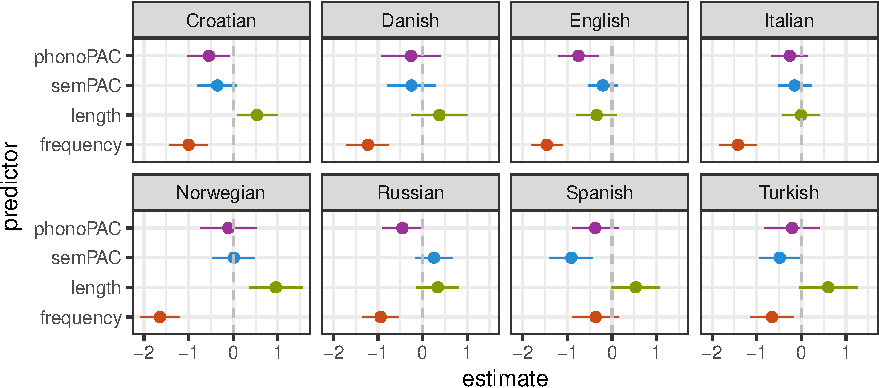
\includegraphics{figs/regressions_img-1} 

}

\caption{\label{fig:regressions_img}Estimates of predictor coefficients by language. Values above 0 indicate a positive relationship (e.g. longer words tend to have a higher AoA), while values below 0 indicate a negative relationship (e.g. words with higher frequency tend to have a lower AoA). Ranges indicate 95\% confidence intervals.}\label{fig:regressions_img}
\end{figure*}
\end{CodeChunk}

\subsection{Comparison to other known predictors of age of
acquisition}\label{comparison-to-other-known-predictors-of-age-of-acquisition}

We saw that the way semantic and phonological information is structured
in the learning environment (i.e., PAC) contribute to noun learning
across languages. However, we know that other factors influence learning
as well (e.g., Braginsky et al., 2016). In what follows, we will
investigate how semantic and phonological connectivity interact with two
other factors. The first one is word frequency, a well studied factor
shown to predict the age of acquisition in a reliable fashion (e.g. J.
C. Goodman et al., 2008). The second factor is word length, which
correlates with phonological connectivity (Pisoni, Nusbaum, Luce, \&
Slowiaczek, 1985).

Since PAT was uninformative, we dropped it from this analysis. Thus, we
no longer needed to fit the growth model month-by-month as in the
previous section. In fact, word utilities in the case of PAC are fixed,
they do not depend on previously learned words. A more direct way to
assess and compare the contribution of PAC in relation to other factors
is through conducting linear regressions, where connectivity in the
learning environment (at both the phonological and semantic level),
frequency and length predict the age of acquisition.

We used the frequency estimates from Braginsky et al. (2016) where
unigram counts were derived based on CHILDES corpora in each language.
For each word, counts included words that shared the same stem (e.g.,
cats counts as cat), or words that were synonymous (e.g.~father counts
as daddy). For word length, we used our generated IPA transcription.

We conducted two analyses. We fit a linear regression for each language,
and we fit a linear mixed-effect to all the data pooled across
languages, with language as a random effect. Figure
\ref{fig:regressions_img} shows the coefficient estimate for each
predictor in each language, and figure \ref{fig:regressions_all_img}
shows the coefficient estimates for all languages combined (all
predictors were centered and scaled). The findings were as follows.
Overall, frequency is the largest and most consistent predictor of age
of acquisition. Word length predicts learning in some languages such as
Croatian and Norwegian, but not in others (including English). It
remains, however, a significant predictor in the global model. As for
the factors of interest, i.e., semantic and phonological connectivity,
we also found cross-linguistic differences. The phonological
connectivity contributes to learning in languages such as Croatian,
English and Russian, whereas semantic connectivity contributes to
learning in Turkish, Spanish and to some extent in Croatian, but
interestingly not in
English\footnote{Semantic connectivity does not explain variance in English data beyond that explained by phonological connectivity, frequency and length. This contrasts with the original finding in Hills et al. 2009. However, in this previous study, semantic connectivity was not tested in a model that included both frequency and length as covariates. Another important difference is the number of words tested. Our study uses a larger set of nouns.}.
Despite this cross-linguistic variation, both phonological and semantic
connectivity remain significant predictors in the global model.

\section{Discussion}\label{discussion}

The present study provided a comprehensive analysis of how lexical
connectivity influences the age of acquisition of nouns in toddlers. We
compared two network growth scenarios and assessed the relative
contribution of phonological and semantic information in 8 languages.
Part of the findings largely replicate the results obtained in Hills et
al. (2009), i.e., semantic networks (based on free associations) grow by
preferential acquisition, not by preferential attachment. Another
finding was that phonological networks also grow primarily by
preferential acquisition, especially when both scenarios (PAT and PAC)
were pitted against each other in the same model. These findings
generalize well across languages. Moreoever, both semantic and
phonological connectivity in the learning environment (i.e., PAC)
predict growth in a consistent way across many languages. However, when
pitted against other known predictors of age of acquisition (word
frequency and length), the effect of word connectivity shows a
cross-linguistic variation, predicting learning in some languages, but
not in others. Despite this cross-lingusitic variation, both
phonological and semantic connectivity contribute to the overall
learning (when data is pooled across languages).

\begin{CodeChunk}
\begin{figure}[H]

{\centering 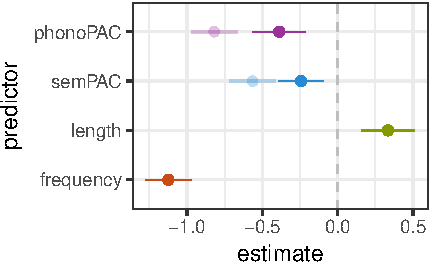
\includegraphics{figs/regressions_all_img-1} 

}

\caption{\label{fig:regressions_all_img}Estimates of predictor coefficients in the combined model pooling across languages . Ranges indicate 95\% confidence intervals. Fade color indicates estimates of PAC predictors in a model that does not include frequency and length as covariates.}\label{fig:regressions_all_img}
\end{figure}
\end{CodeChunk}

A major results of the study is that children start by learning words
that have high phonological and semantic similarity with a variety of
other words in the learning environment, not in the child's available
lexicon. This suggests that children are sensitive to connectivity even
without having first acquired the connected words. How can children
indirectly detect highly connected words, and why would such words be
more readily learned? In the semantic case, free association can be
predicted through the patterns of word co-occurrence (Griffiths,
Steyvers, \& Tenenbaum, 2007), meaning that highly connected words tend
to be the words that co-occur with many other words in various contexts.
One possibility, suggested by Hills et al. (2010), is that the referents
of such words are more easily disambiguated from other potential
referents. Such effect was demonstrated by cross-situational learning
experiments (Smith \& Yu, 2008). In the phonological case, connectivity
is inherently correlated with phonotactic probability (Vitevitch, Luce,
Pisoni, \& Auer, 1999). That is, highly connected words tend to be made
of frequent sound sequences. We know even infant (whose vocabulary is
still very rudimentary) develop a sensitivity for high frequency sound
sequences in the ambient language (Jusczyk, Luce, \& Charles-Luce,
1994). Interestingly, it was shown that phonotactic probability
facilitates learning and recognition of novel words in toddlers and
preschoolers (MacRoy-Higgins, Shafer, Schwartz, \& Marton, 2014;
Storkel, 2001). Thus, children's ability to keep track of co-occurrence
statistics (both at the semantic and phonological level) might explain
their sensitivity and preference for highly connected words in the
learning envirnoment.

Finally, this study shares a number of limitations with previous studies
using similar datasets. For instance, we used normative age of
acquisition. However, individual children may follow different learning
trajectories. The use of longitudinal data would allow us to assess how
the aggregate behavior relates to these individual trajectories (e.g.,
typical vs.~late talkers, Beckage et al., 2011). Moreover, the results
obtained in this study provide correlational but not causal evidence.
Thus, conclusions drawn from our network analysis would require parallel
evidence, especially from controlled behavioral experiments.

\vspace{1em}

\fbox{\parbox[b][][c]{7.3cm}{\centering All data and code for these analyses are available at\ \url{https://github.com/afourtassi/networks}}}
\vspace{1em}

\section{Acknowledgements}\label{acknowledgements}

This work was supported by a post-doctoral grant from the Fyssen
Foundation.

\section{References}\label{references}

\setlength{\parindent}{-0.1in} \setlength{\leftskip}{0.125in} \noindent

\hypertarget{refs}{}
\hypertarget{ref-barabasi99}{}
Barabasi, A.-L., \& Albert, R. (1999). Emergence of scaling in random
networks. \emph{Science}, \emph{286}(5439), 509--512.

\hypertarget{ref-beckage2011}{}
Beckage, N. M., Smith, L., \& Hills, T. T. (2011). Small worlds and
semantic network growth in typical and late talkers. \emph{PLOS ONE},
\emph{6}(5), 1--6.

\hypertarget{ref-braginsky2016}{}
Braginsky, M., Yurovsky, D., Marchman, V. A., \& Frank, M. C. (2016).
From uh-oh to tomorrow: Predicting age of acquisition for early words
across languages. In \emph{Proceedings of the 38th Annual Conference of
the Cognitive Science Society}.

\hypertarget{ref-engelthaler2017}{}
Engelthaler, T., \& Hills, T. T. (2017). Feature biases in early word
learning: Network distinctiveness predicts age of acquisition.
\emph{Cognitive Science}, \emph{41}, 120--140.

\hypertarget{ref-frank2017}{}
Frank, M. C., Braginsky, M., Yurovsky, D., \& Marchman, V. A. (2017).
Wordbank: An open repository for developmental vocabulary data.
\emph{Journal of Child Language}, \emph{44}(3), 677--694.

\hypertarget{ref-goodman2008}{}
Goodman, J. C., Dale, P. S., \& Li, P. (2008). Does frequency count?
Parental input and the acquisition of vocabulary. \emph{Journal of Child
Language}, \emph{35}(3), 515--531.

\hypertarget{ref-dippl}{}
Goodman, N., \& Stuhlmüller, A. (2014). The Design and Implementation of
Probabilistic Programming Languages. \url{http://dippl.org}.

\hypertarget{ref-griffiths07}{}
Griffiths, T. L., Steyvers, M., \& Tenenbaum, J. B. (2007). Topics in
semantic representation. \emph{Psychological Review}, \emph{114}(2),
2007.

\hypertarget{ref-hills2010}{}
Hills, T. T., Maouene, J., Riordan, B., \& Smith, L. B. (2010). The
associative structure of language: Contextual diversity in early word
learning. \emph{Journal of Memory and Language}, \emph{63}(3), 259--273.

\hypertarget{ref-hills2009}{}
Hills, T. T., Maouene, M., Maouene, J., Sheya, A., \& Smith, L. (2009).
Longitudinal analysis of early semantic networks: Preferential
attachment or preferential acquisition? \emph{Psychological Science},
\emph{20}(6), 729--739.

\hypertarget{ref-jusczyk1994}{}
Jusczyk, P. W., Luce, P. A., \& Charles-Luce, J. (1994). Infant's
sensitivity to phonotactic patterns in the native language.
\emph{Journal of Memory and Language}, \emph{33}(5), 630--645.

\hypertarget{ref-higgins2014}{}
MacRoy-Higgins, M., Shafer, V. L., Schwartz, R. G., \& Marton, K.
(2014). The influence of phonotactic probability on word recognition in
toddlers. \emph{Child Language Teaching and Therapy}, \emph{30}(1),
117--130.

\hypertarget{ref-nelson1998}{}
Nelson, D. L., McEvoy, C. L., \& Schreiber, T. A. (1998). The University
of South Florida word association, rhyme, and word fragment norms.
Retrieved from \url{http://w3.usf.edu/FreeAssociation/}

\hypertarget{ref-pisoni1985}{}
Pisoni, D. B., Nusbaum, H. C., Luce, P. A., \& Slowiaczek, L. M. (1985).
Speech perception, word recognition and the structure of the lexicon.
\emph{Speech Communication}, \emph{4}(1), 75--95.

\hypertarget{ref-smith2008}{}
Smith, L., \& Yu, C. (2008). Infants rapidly learn word-referent
mappings via cross-situational statistics. \emph{Cognition},
\emph{106}(3), 1558--1568.

\hypertarget{ref-stella2017}{}
Stella, M., Beckage, N. M., \& Brede, M. (2017). Multiplex lexical
networks reveal patterns in early word acquisition in children.
\emph{Scientific Reports}, \emph{7}.

\hypertarget{ref-steyvers2005}{}
Steyvers, M., \& Tenenbaum, J. B. (2005). The large-scale structure of
semantic networks: Statistical analyses and a model of semantic growth.
\emph{Cognitive Science}, \emph{29}(1), 41--78.

\hypertarget{ref-stokes2010}{}
Stokes, S. F. (2010). Neighborhood density and word frequency predict
vocabulary size in toddlers. \emph{Journal of Speech, Language, and
Hearing Research}, \emph{53}(3), 670--683.

\hypertarget{ref-storkel2001}{}
Storkel, H. L. (2001). Learning new words: Phonotactic probability in
language development. \emph{Journal of Speech, Language, and Hearing
Research}, \emph{44}(6), 1321--1337.

\hypertarget{ref-storkel2009}{}
Storkel, H. L. (2009). Developmental differences in the effects of
phonological, lexical and semantic variables on word learning by
infants. \emph{Journal of Child Language}, \emph{36}(2), 29--321.

\hypertarget{ref-vitevitch1999}{}
Vitevitch, M. S., Luce, P. A., Pisoni, D. B., \& Auer, E. T. (1999).
Phonotactics, neighborhood activation, and lexical access for spoken
words. \emph{Brain and Language}, \emph{68}(1), 306--311.

\end{document}
